\begin{frame}\frametitle{Introduction. The Standard Model}
\scriptsize
About the Standard Model
\end{frame}%{Introduction. The Standard Model}

\begin{frame}\frametitle{Theory. Proton-Proton Collisions}
%\begin{figure}[htb]
%  \begin{center}
%    {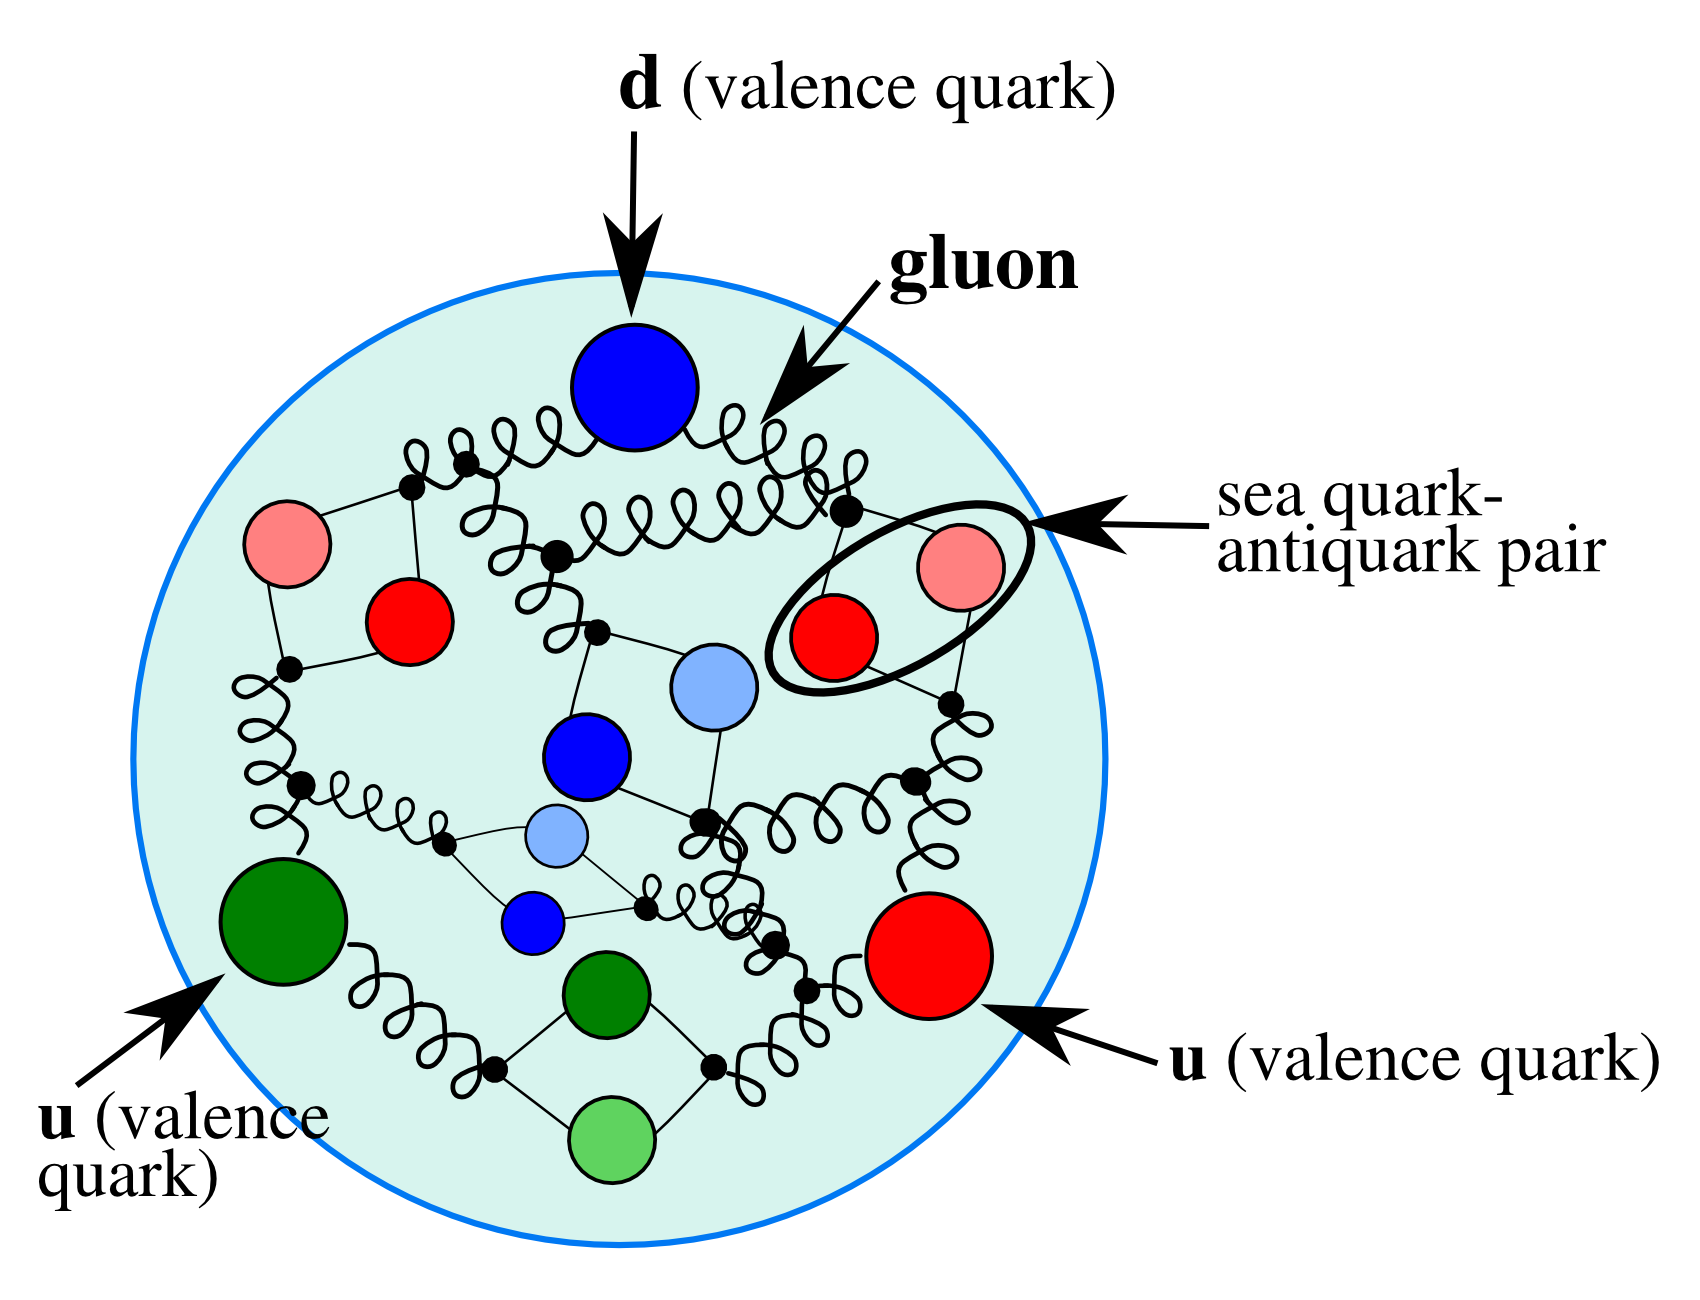
\includegraphics[width=0.45\textwidth]{../figs/Intro/protonStructure.png}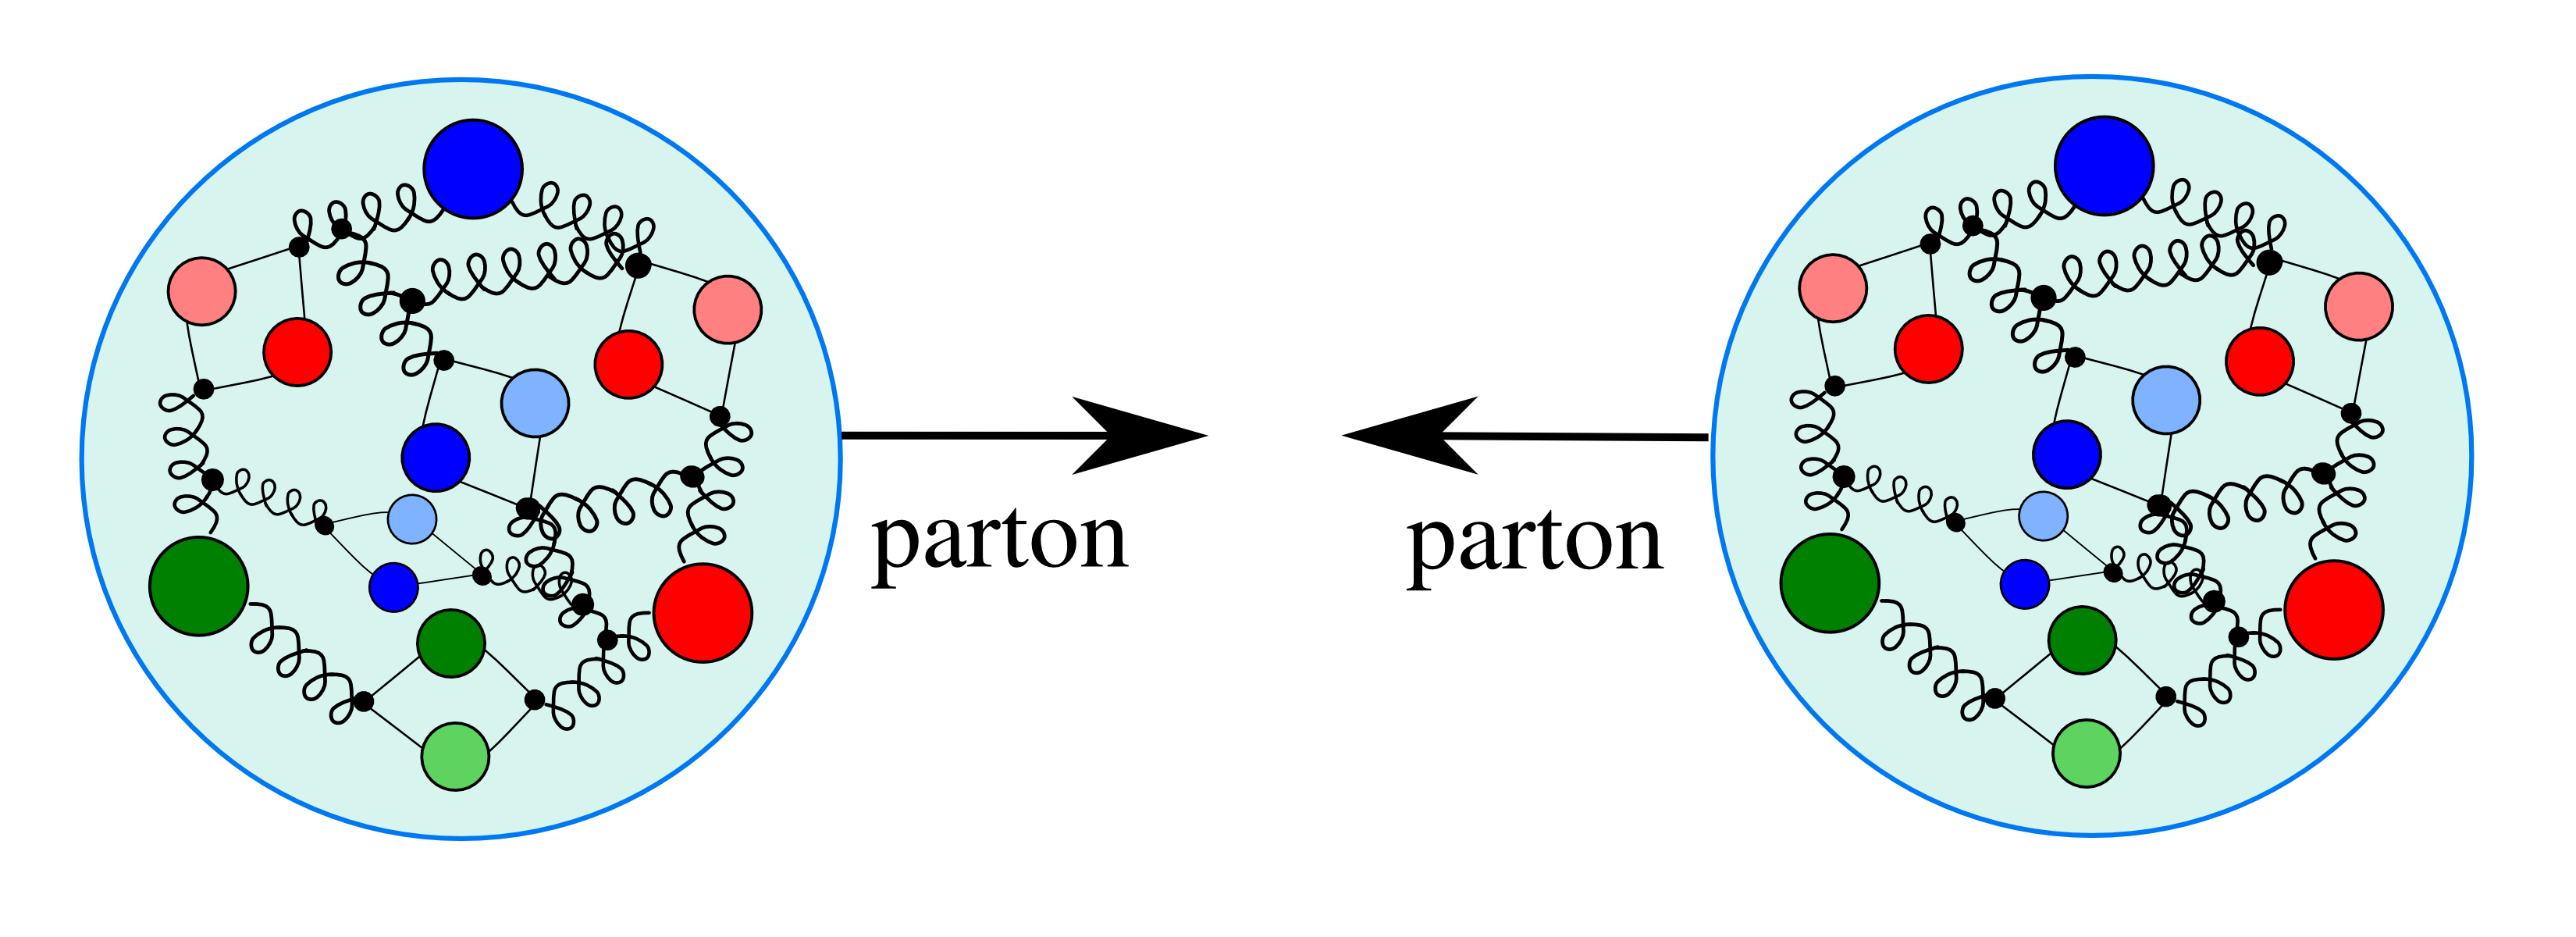
\includegraphics[width=0.45\textwidth]{../figs/Intro/ppCollision.png}}
%  \end{center}
%\end{figure}
\end{frame}%{Proton-Proton Collisions}

\begin{frame}\frametitle{Theory. $W\gamma\rightarrow l\nu\gamma$}

\scriptsize
ISR: initial state radiation\\
FSR: final state radiation\\
TGC: triple gauge coupling

   \begin{figure}[htb]
      \begin{center}
        \scriptsize
          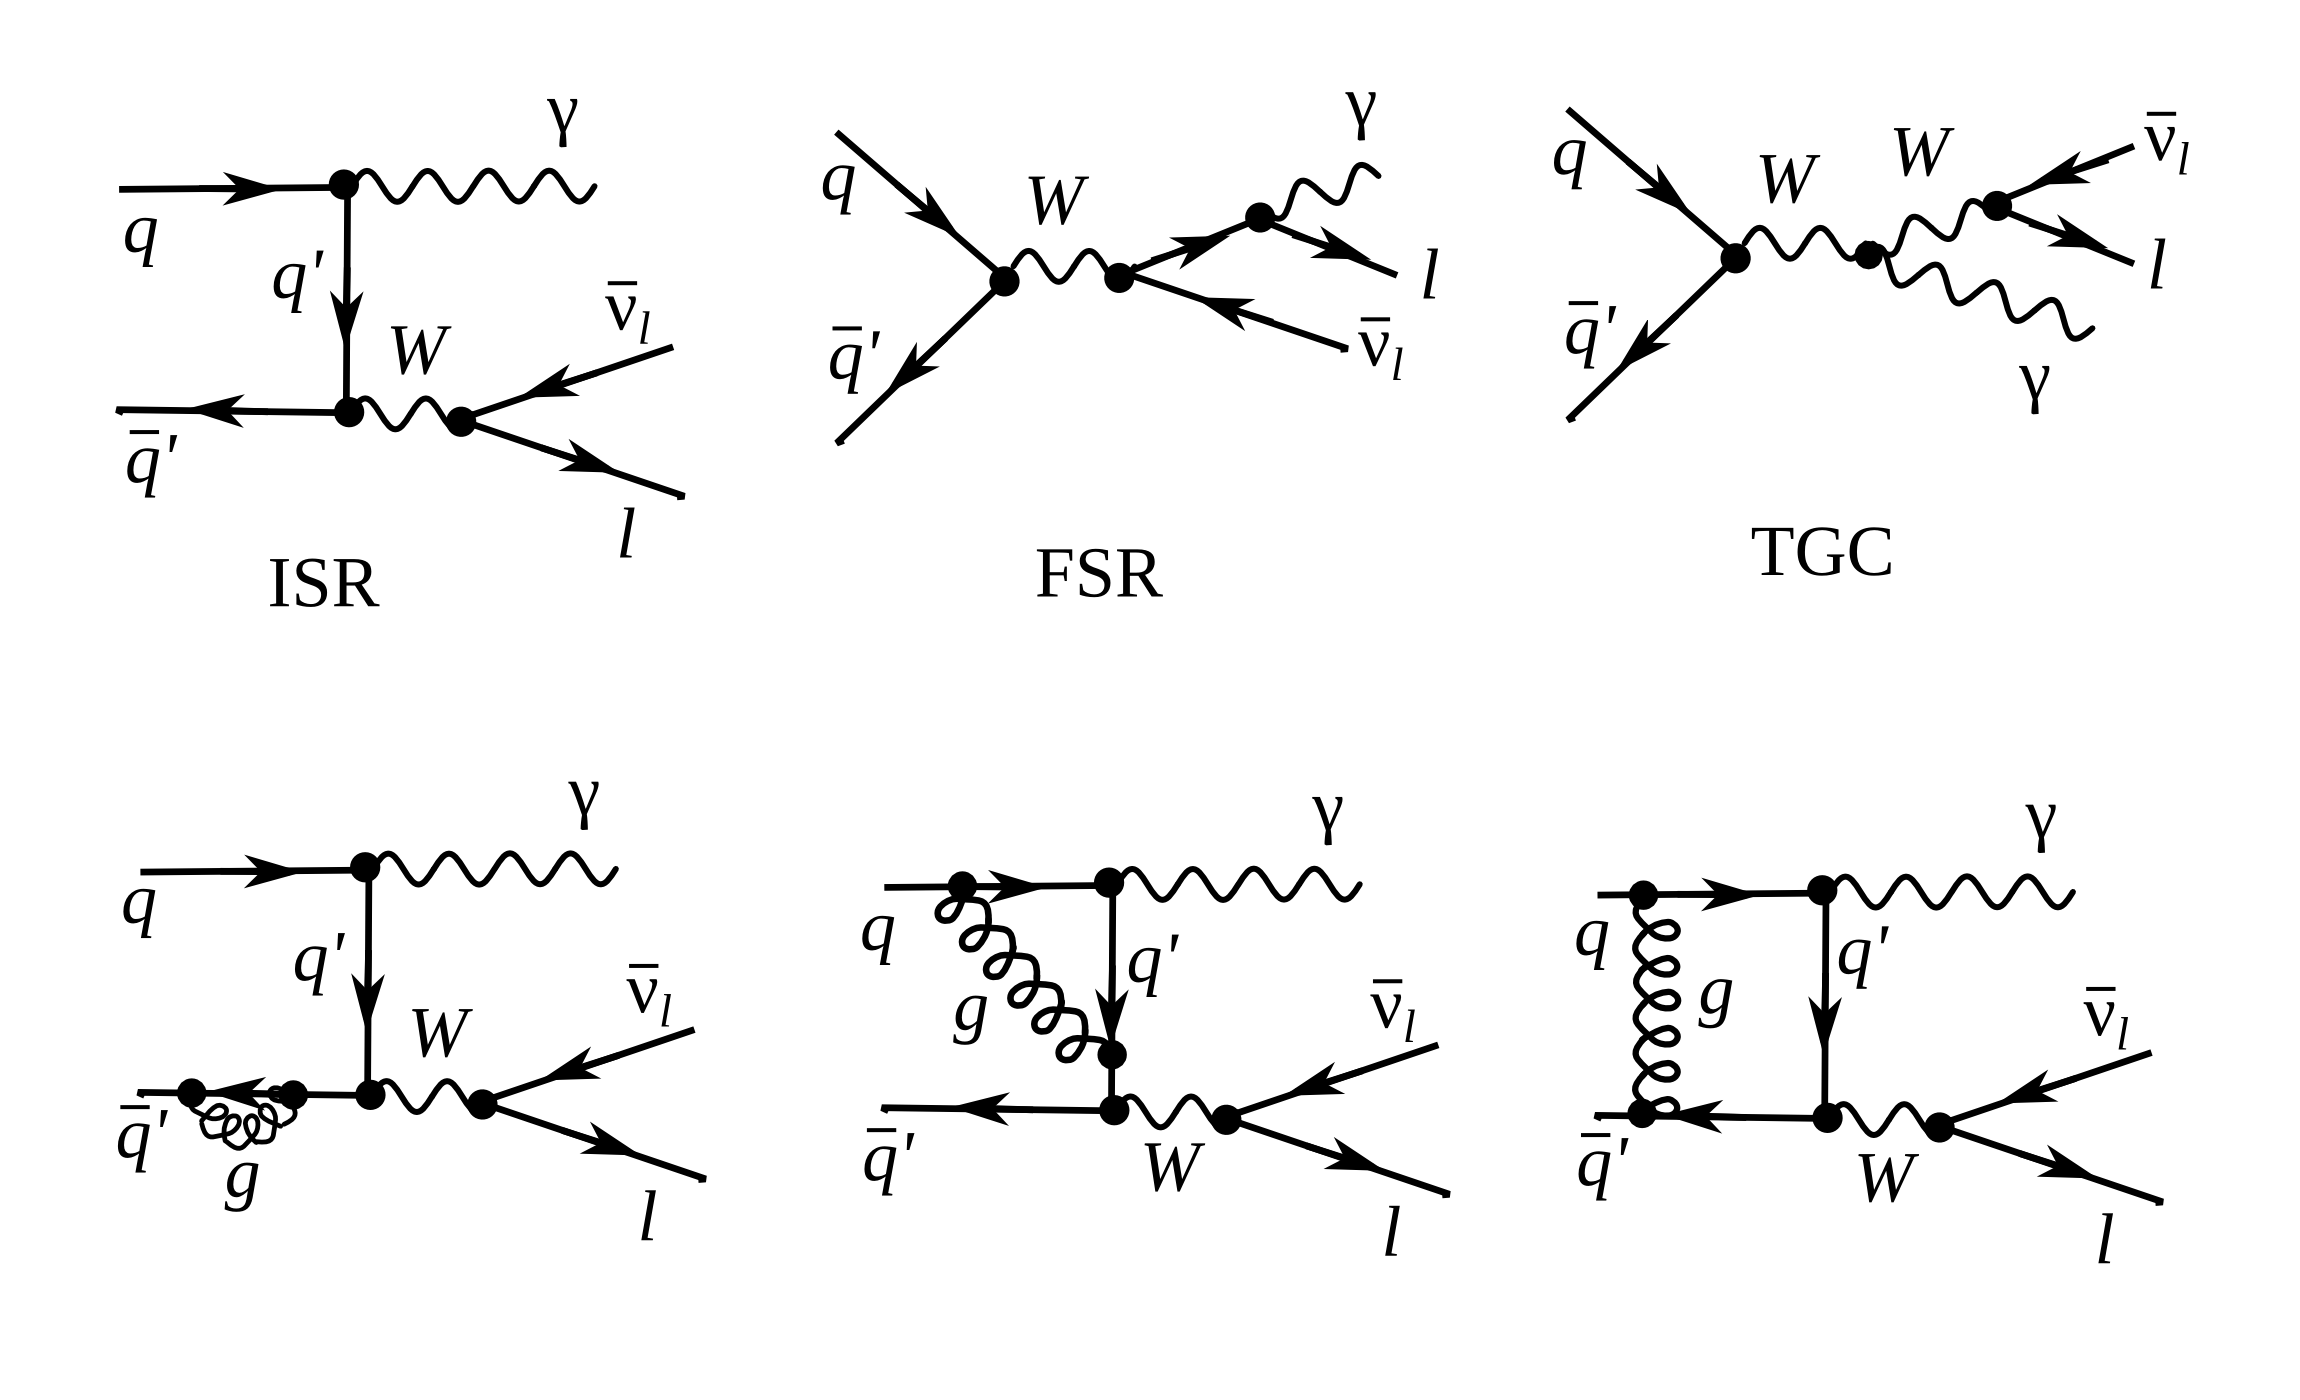
\includegraphics[width=0.95\textwidth]{../figs/WgAbout/feynmWg_LO_NLO.png}
%          \caption{\scriptsize{The Feynman diagrams. ISR(x2), FSR, and TGC.}}
       \end{center}
    \end{figure}

  \begin{itemize}
    \scriptsize
    \item test Standard Model;
    \item search for aTGC.
  \end{itemize}
\end{frame}%{Theory. $W\gamma\rightarrow l\nu\gamma$}
